\documentclass[10pt,a4paper]{article}
\usepackage[utf8]{inputenc}

\usepackage{amsmath}
\usepackage{amsfonts}
\usepackage{amssymb}
\usepackage{graphicx}
\usepackage{listings}

\lstset{numbers=left,
	title=\lstname,
	numberstyle=\tiny,
	breaklines=true,
	tabsize=4,
	language=Python,
	morekeywords={with,super,as},,
	frame=single,
	basicstyle=\footnotesize\tt,
	commentstyle=\color{comment},
	keywordstyle=\color{keyword},
	stringstyle=\color{string},
	backgroundcolor=\color{background},
	showstringspaces=false,
	numbers=left,
	numbersep=5pt,
	literate=
		{�}{{\ae}}1
		{�}{{\aa}}1
		{�}{{\o}}1
		{�}{{\AE}}1
		{�}{{\AA}}1
		{�}{{\O}}1
	}
\usepackage{setspace}
\doublespacing
\usepackage{bm}
\usepackage{hyperref}

\begin{document}
\begin{center}
{\LARGE\bf
FYS4150\\
Project 2, deadline October 2.
}
 
\includegraphics[scale=0.1]{uio.png}\\
Authors: Robin D. Kifle, Sander W. Losnedahl and Vemund S. Thorkildsen\\
University of Oslo, Autumn 2017

{\LARGE\bf Abstract}
\end{center}
\newpage

\begin{center}
{\LARGE\bf Introduction}
\end{center}
The problem we will deal with in this project is of quantum mechanical nature. As none of the three authors have had any quantum mechanics courses we will focus on the mathematical and numerical side of this problem. In this project we are going to develop our own eigenvalue-solver by using Jacobi's method. We will study two different cases, the first is for one electron moving in a harmonic oscillator. The second case is for two electrons moving in a harmonic oscillator with and without repulsive coulomb interaction.
\newpage'

\begin{center}
{\LARGE\bf Method}
\end{center}
To create our eigenvalue solver we first have to take a look at the matrix at hand, to get an understanding of the problem.

$$
  -\frac{d^2}{d\rho^2} u(\rho) + \rho^2u(\rho)  = \lambda u(\rho) .
$$

\noindent This equation will be solved numerically, and has given eigenvalues $\lambda_0=3$, $\lambda_1=7$ and $\lambda_2=11$. We can use the expression for the second derivative to rewrite this. This expression is in our case given by:

$$
 u''=\frac{u(\rho+h) -2u(\rho) +u(\rho-h)}{h^2} +O(h^2)
$$
\noindent
The last part of this expression, namely $O(h^2$, is the truncation error and will not be used further. Bu using the first part, our expression now looks like this:

$$
\frac{-u(\rho_i+h) +2u(\rho_i) -u(\rho_i-h)}{h^2}+\rho_i^2u(\rho_i)  = \lambda u(\rho_i)
$$

$$
\frac{-u_{i+1} +2u_i -u_{i-1}}{h^2}+\rho_i^2u_i= \lambda u_i
$$

\noindent Our $h$ is given by $h=\frac{\rho_n - \rho_0}{n}$, as we want our $\rho_i$ to vary with step length $h$. By using this $h$, $\rho_i$ will take the form: $\rho_i = \rho_o + ih$. The oscillator potential is given by $(\rho_i)^2$ and will be denoted as $V_i$ in the rest of this article. Now we have everything we need to rearrange this problem as a a matrix eigenvalue problem. \\
\\
From our expression it is easy to see that the matrix we are looking for takes the negative of element $i+1$ and $i-1$, divided by the step length squared. It also need to take two times the positive of element $i$ divided by $h^2$ plus element $i$ multiplied by the oscillator potential $V_i$. This means that we are once again faced by a problem that involves a tridiagonal matrix.

\begin{center}
Main diagonal = $\frac{2}{h^2} + V_i$, first diagonal above and below = $-\frac{1}{h^2}$
\end{center}

\noindent On matrix form this looks like:

\begin{center}


$
 \begin{bmatrix}
 \frac{2}{h^2}+V_1 & -\frac{1}{h^2} & 0   & 0    & \dots  &0     & 0 \\
 -\frac{1}{h^2} & \frac{2}{h^2}+V_2 & -\frac{1}{h^2} & 0    & \dots  &0     &0 \\
  0   & -\frac{1}{h^2} & \frac{2}{h^2}+V_3 & -\frac{1}{h^2}  &0       &\dots & 0\\
  \dots  & \dots & \dots & \dots  &\dots      &\dots & \dots\\
  0   & \dots & \dots & \dots  &\dots  &\dots & \dots\\
 0   & \dots & \dots & \dots  &\dots       & \dots & \frac{2}{h^2}+V_{N-1}
             \end{bmatrix}
             \begin{bmatrix}
             u_0\\
             u_1\\
             u_2\\
             \dots\\
             \dots\\
             u_n\\
             \end{bmatrix} =\lambda
             \begin{bmatrix}
              u_0\\
             u_1\\
             u_2\\
             \dots\\
             \dots\\
             u_n\\
             \end{bmatrix}
$
\end{center}
We are going to solve this by using a Jacobi rotation algorithm. This uses a lot of similarity transformations. As long as:
$$v_j^Tv_i=\delta_{i j}$$
$$U^TU=I$$
The transformations can be shown to preserve the dot product and orthogonality by multiplying with the transpose of the matrix:
$$w=Uv$$
$$w^Tw=(Uv)^TUv=v^TU^TUv=v^Tv=\delta_{i j}$$






\newpage

\begin{center}
{\LARGE\bf Results}
\end{center}


\begin{center}
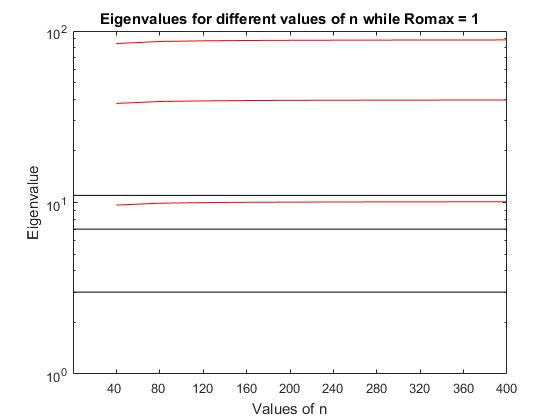
\includegraphics[scale=0.65]{rho1.jpg}
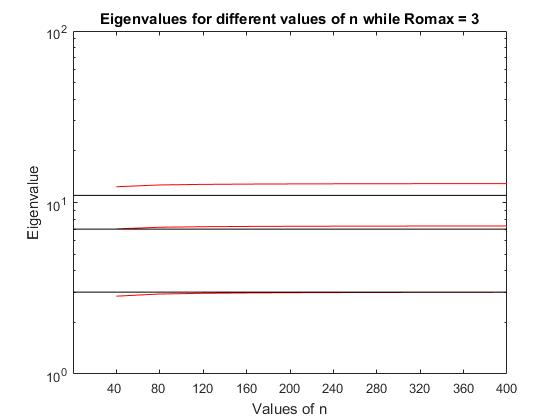
\includegraphics[scale=0.65]{rho3.jpg}
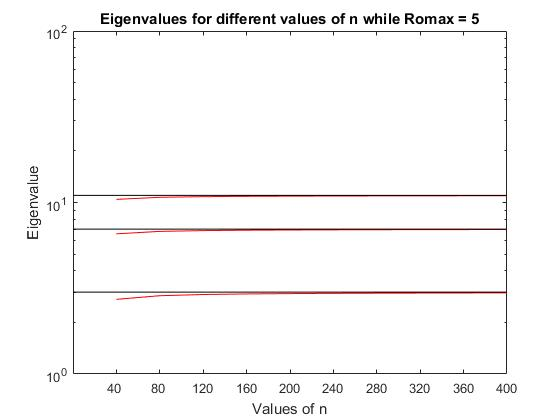
\includegraphics[scale=0.65]{rho5.jpg}
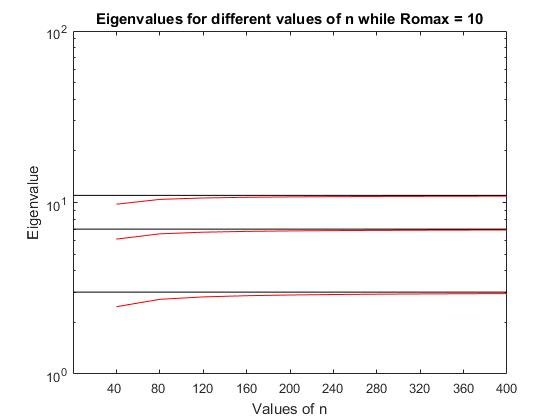
\includegraphics[scale=0.65]{rho10.jpg}
\end{center}



\newpage

\begin{center}
{\LARGE\bf Discussion}
\end{center}
\newpage

\begin{center}
{\LARGE\bf Concluding remarks}
\end{center}
\end{document}
